% Created 2023-02-12 Sun 13:35
% Intended LaTeX compiler: pdflatex
\documentclass[sigconf]{acmart}
\usepackage[utf8]{inputenc}
\usepackage[T1]{fontenc}
\usepackage{graphicx}
\usepackage{float}
\usepackage[export]{adjustbox}
\usepackage{grffile}
\usepackage{longtable}
\usepackage{wrapfig}
\usepackage{rotating}
\usepackage[normalem]{ulem}
\usepackage{amsmath}
\usepackage{textcomp}
\usepackage{amssymb}
\usepackage{capt-of}
\usepackage{hyperref}
\usepackage{pmboxdraw}
\usepackage{newunicodechar}
\usepackage{anyfontsize}
\usepackage{pifont}
\usepackage{fancyvrb}
\date{\today}

\setcopyright{acmcopyright}
\copyrightyear{2023}
\acmYear{2023}
\acmDOI{XXXXXXX.XXXXXXX}

\acmConference[Conference acronym 'ELS]{European Lisp Symposium}{April 24--25,
  2023}{Amsterdam, NL}


\title{GRASP: An Extensible Tactile Interface for Editing S-expressions}
\hypersetup{
 pdfauthor={Panicz Maciej Godek},
 pdftitle={GRASP: An Extensible Tactile Interface for Editing S-expressions},
 pdfkeywords={},
 pdfsubject={},
 pdfcreator={Emacs 27.1 (Org mode 9.3)}, 
 pdflang={English}}
\newunicodechar{─}{\textSFx}
\newunicodechar{│}{\textSFxi}
\newunicodechar{╭}{\textSFi}
\newunicodechar{╰}{\textSFii}
\newunicodechar{╮}{\textSFiii}
\newunicodechar{╯}{\textSFiv}

\newunicodechar{┈}{\textSFx}
\newunicodechar{┊}{\textSFxi}
\newunicodechar{❝}{{\fontsize{6.8}{0}\ding{125}}}
\newunicodechar{❞}{{\fontsize{6.8}{0}\ding{126}}}

\newenvironment{Snippet}{\Verbatim[samepage=true]}{\endVerbatim}

\begin{document}

\author{Panicz Maciej Godek}
\email{godek.maciek@gmail.com}

\begin{abstract}

GRASP is a Scheme-based extensible computational environment
designed to work with S-expressions on touch screens. It features
a powerful extension mechanism as well as a subsystem for
handling gesture-based input. It is implemented in Kawa Scheme,
and can be compiled as an Android application as well as run
on a desktop windowing environment and inside of terminal
emulators.

GRASP is still a work-in-progress application, so the purpose
of the demo is:
\begin{enumerate}
\item to show the current state of the application;
\item to convey the ultimate vision behind GRASP;
\item to present the development plan and methodology, and optionally:
\item to describe the hitherto history of the development.
\end{enumerate}

The presentation of GRASP in this paper is written as if
all of its features were already implemented. The omissions
are presented in a separate section.

\end{abstract}


\begin{CCSXML}
  <ccs2012>
  <concept>
  <concept_id>10011007.10011006.10011066.10011069</concept_id>
  <concept_desc>Software and its engineering~Integrated and visual development environments</concept_desc>
  <concept_significance>500</concept_significance>
  </concept>
  <concept>
  <concept_id>10003120.10003145.10003151.10011771</concept_id>
  <concept_desc>Human-centered computing~Visualization toolkits</concept_desc>
  <concept_significance>300</concept_significance>
  </concept>
  <concept>
  <concept>
  <concept_id>10003120.10003138.10003140</concept_id>
  <concept_desc>Human-centered computing~Ubiquitous and mobile computing systems and tools</concept_desc>
  <concept_significance>300</concept_significance>
  </concept>
  <concept_id>10010147.10010371.10010387.10010391</concept_id>
  <concept_desc>Computing methodologies~Graphics input devices</concept_desc>
  <concept_significance>100</concept_significance>
  </concept>
  </ccs2012>
\end{CCSXML}

\ccsdesc[500]{Software and its engineering~Integrated and visual development environments}
\ccsdesc[300]{Human-centered computing~Visualization toolkits}
\ccsdesc[300]{Human-centered computing~Ubiquitous and mobile computing systems and tools}
\ccsdesc[100]{Computing methodologies~Graphics input devices}

\keywords{visual programming, touchscreen-based editing, interactive programming,
structual editing}

\maketitle

\section{The concept of GRASP}

GRASP\footnote{GRASP is an open-source project hosted at
  \url{https://github.com/panicz/grasp}} is a tactile-first
structural editor for S-expressions.
Its design is based on representing S-expressions as
nestable boxes. The boxes are rendered so that their left 
and right edge resemble -- respectively -- opening and closing 
parentheses.

When displayed in a terminal, a Lisp program edited in GRASP
might look like this\footnote{Some recordings presenting various
  prototypes of GRASP can be watched on the author's youtube channel:
  \url{https://www.youtube.com/channel/UCt4u6WQDy2yjXz6eXCcyijQ}}:

\begin{Snippet}
╭        ╭     ╮                       ╮
│ define │ ! n │                       │
│        ╰     ╯                       │
│ ❝ ┈┈┈┈┈┈┈┈┈┈┈┈┈┈┈┈┈┈┈┈┈┈┈┈┈┈┈┈┈┈┈┈ • │
│ ┊ Computes the product 1*...*n.    ┊ │
│ ┊ It represents the number of per- ┊ │
│ ┊ mutations of an n-element set.   ┊ │
│ • ┈┈┈┈┈┈┈┈┈┈┈┈┈┈┈┈┈┈┈┈┈┈┈┈┈┈┈┈┈┈┈┈ ❞ │
│   ╭    ╭        ╮                 ╮  │
│   │ if │ <= n 0 │                 │  │
│   │    ╰        ╯                 │  │
│   │                               │  │
│   │       1                       │  │
│   │                               │  │
│   │       ╭     ╭   ╭       ╮ ╮ ╮ │  │
│   │       │ * n │ ! │ - n 1 │ │ │ │  │
╰   ╰       ╰     ╰   ╰       ╯ ╯ ╯ ╯  ╯
╭      ╭             ╮          ╮       
│ e.g. │ factorial 5 │ ===> 120 │       
╰      ╰             ╯          ╯       
\end{Snippet}

which corresponds to the following program text:

\begin{Snippet}
(define (! n)
"Computes the product 1*...*n.
It represents the number of per-
mutations of an n-element set."
  (if (<= n 0)
      1
      (* n (! (- n 1))))) 
(e.g. (factorial 5) ===> 120)
\end{Snippet}

The left and right parentheses play different roles in 
tactile editing: the left parenthesis is used for moving
(if pressed once) or copying (if pressed twice) an expression,
whereas the right parenthesis is used for resizing an expression.

An expression which is currently being moved can be deleted
by throwing it off the surface quickly. Likewise, moving
a finger quickly while the expression is being resized
causes the box to be spliced into its parent (this feature
is sometimes referred to as ``pulling-the-rug splicing'').

In addition to boxes, GRASP offers four other types
of objects: atoms, texts, extensions and comments.

Atoms are things like symbols, numbers, characters
or Boolean values in Lisp. They support touch
gestures in a similar way as the left parenthesis
of a box: single touch causes them to be dragged,
whereas double touch causes their copy to be dragged.

The text type corresponds to strings. They are 
displayed inside boxes with quotation marks
on their corners. The roles of the quotation
marks are analogous to the left and the right
parenthesis: the left one can be used to
move the text within the expression tree,
remove it or copy, while the right one can be used
to change the shape of a text.

Comments in the Scheme programming language come in
three flavors, all of which are supported by GRASP:
\begin{itemize}
\item line comments, which span until the end of a given line;
\item block comments, which are similar to text;
\item expression comments, which comment out a single expression.
\end{itemize}

Comments are invisible to the operations
on the document, such as \texttt{car} or \texttt{cdr}. 
Other than that, line and block comments are similar to text.

The last type of objects supported by the editor
are extensions. The list of extensions is open-ended.
Expressions are sometimes referred to as ``magic boxes'',
because they are boxes which define their own rules
of interaction.

A simple example of an extension is a button.
If it is loaded, the expression

\begin{Snippet}
(Button label: "Press me" 
	action: (lambda () (WARN "button pressed")))
\end{Snippet}

can be rendered as a button, and respond
to touch events with the invocation of its
action callback.

The terminal client of GRASP would display
it in the following manner:

\begin{Snippet}
╭───────────╮
│ Press me! │
╰───────────╯
\end{Snippet}

A more advanced extension -- coming from an earlier
prototype of GRASP -- allows to display graphs represented
in the form of neighbour list as an actual graph:

\begin{figure}[H]
  \centering%
  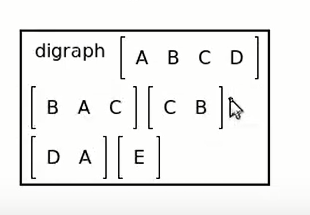
\includegraphics[width=.45\linewidth,frame]{digraph-1}\hfill%
  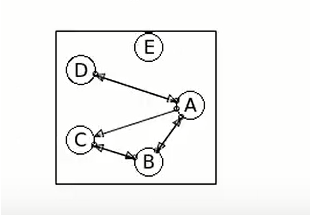
\includegraphics[width=.45\linewidth,frame]{digraph-2}\hfill%
\end{figure}

Extensions are meant to be user-definable, but
the exact API for defining them is subject to
an ongoing research.

Some desired extensions for GRASP include:
\begin{itemize}
\item a drawing editor
\item a graph visualizer/editor
\item a visual evaluator
\item a function plotter
\end{itemize}

and many others.

\subsection{Gesture-based input}

Since devices with touch screens often lack
a proper keyboard, and usually display regrettable
keyboard substitutes on their screens as needed,
GRASP attempts to find a more ergonomic alternative.

One idea is gesture-based input: the user draws
a shape on the screen, and if the shape is recognized,
an appropriate action is performed.

By default, the following shapes are recognized:
\begin{itemize}
\item horizontal line, which splits the panes it's
drawn over vertically into halves
(similar to \texttt{C-x 2} in Emacs)

\begin{figure}[H]
  \centering%
  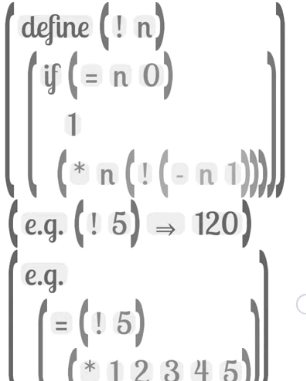
\includegraphics[width=.32\linewidth,frame]{horizontal-line1}\hfill%
  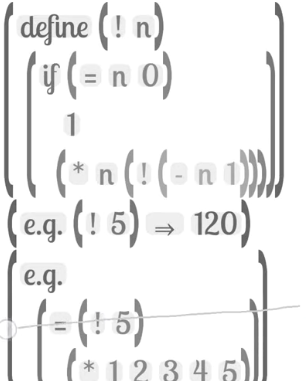
\includegraphics[width=.32\linewidth,frame]{horizontal-line2}\hfill%
  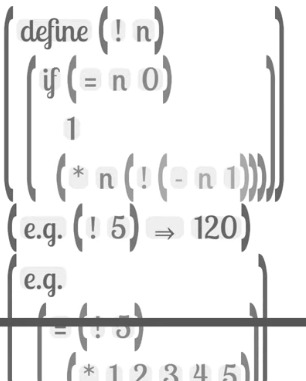
\includegraphics[width=.32\linewidth,frame]{horizontal-line3}\hfill%
\end{figure}

\item vertical line, which splits the panes below
horizontally into halves
(similar to \texttt{C-x 3} in Emacs)

\begin{figure}[H]
  \centering%
  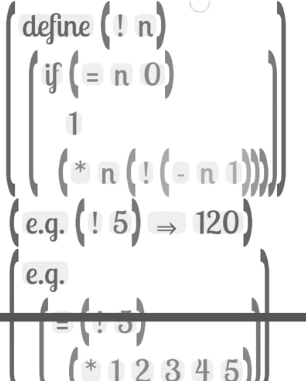
\includegraphics[width=.24\linewidth,frame]{vertical-line1}\hfill%
  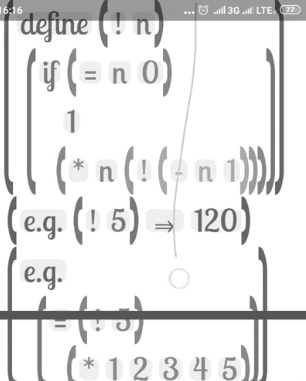
\includegraphics[width=.24\linewidth,frame]{vertical-line2}\hfill%
  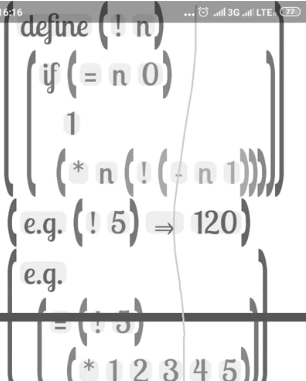
\includegraphics[width=.24\linewidth,frame]{vertical-line3}\hfill%
  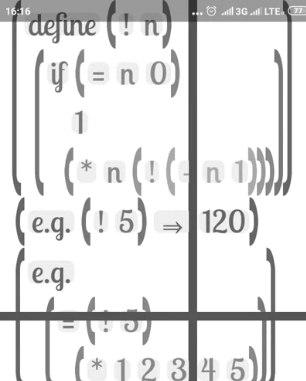
\includegraphics[width=.24\linewidth,frame]{vertical-line4}\hfill%
\end{figure}

\item box gesture, which creates a new box in the
document it's drawn over

\begin{figure}[H]
  \centering%
  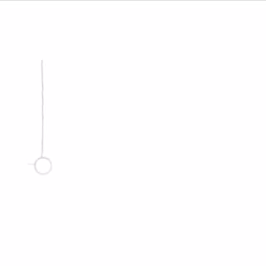
\includegraphics[width=.19\linewidth,frame]{box-2}\hfill%
  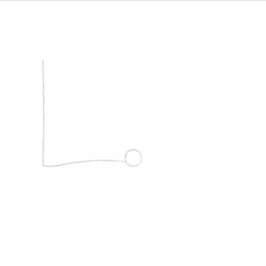
\includegraphics[width=.19\linewidth,frame]{box-3}\hfill%
  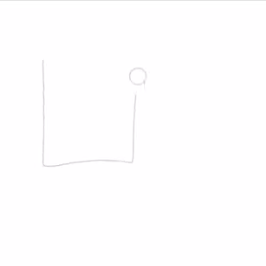
\includegraphics[width=.19\linewidth,frame]{box-4}\hfill%
  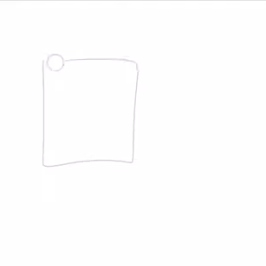
\includegraphics[width=.19\linewidth,frame]{box-5}\hfill%
  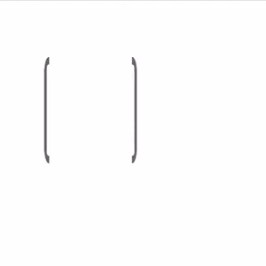
\includegraphics[width=.19\linewidth,frame]{box-6}\hfill%
\end{figure}


%\item an underscore gesture, which creates a new atom
%in the document it's drawn over

\item wedge symbol, which causes the expression
below its blade to be evaluated (similar to
\texttt{C-x C-e} in Emacs' Lisp interaction modes)

\begin{figure}[H]
  \centering%
  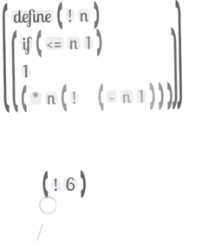
\includegraphics[width=.32\linewidth,frame]{eval-1}\hfill%
  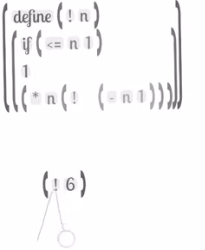
\includegraphics[width=.32\linewidth,frame]{eval-2}\hfill%
  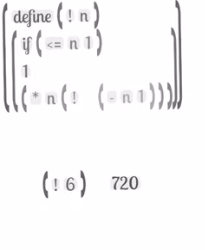
\includegraphics[width=.32\linewidth,frame]{eval-3}\hfill%
\end{figure}

\end{itemize}

Since many touchscreen-equipped devices also
feature accelerometers, GRASP also lets define
motion-based edit operations -- for example, shaking
a device might result in re-indenting the source
code.

\subsection{Keyboard input}

Even though GRASP focuses on tactile editing
and on mobile devices, a lot of effort has been
put into making it a pleasant keyboard editing
experience.

GRASP features a flexible key binding mechanism,
which unites the input systems from its target
environments (Android, terminal and windowing
systems).

By default, it provides the ``Common User Access''
keyboard bindings (ctrl-z for undo, ctrl-c for copy
etc.) and it allows to use keyboard arrows to
navigate cursor over the active document.

Keyboard editing is context-sensitive, so
for example pressing the \texttt{\#\textbackslash[}
key creates a new box, unless the cursor is located on a text element,
in which case the \texttt{\#\textbackslash[} character is inserted verbatim
into text.

Also, extensions are free to interpret
most of the pressed characters as they please.

%% \section{Implementation}

%% GRASP is still a very immature editor, and many 
%% of its implementation details are likely to change. 
%% However, there are certain design decisions that
%% will probably stay fixed throughout the lifetime
%% of GRASP.

%% \subsection{Kawa and JVM inter-operation}

%% GRASP is implemented in -- and intimately coupled
%% to -- Kawa, the implementation of Scheme which runs
%% on the Java Virtual Machine and produces JVM byte code.

%% The main reason for this decision is that JVM
%% byte code can be translated to run on Android,
%% which was both the initial development platform
%% of GRASP, as well as its main target.

%% Kawa Scheme offers a few interesting extensions
%% to facilitate inter-operation with JVM: first,
%% it exposes Java's object model to Scheme
%% (using the \texttt{define-simple-class} special form);
%% second, it extends Scheme with an optional syntax
%% for declaring types, and provides a Java-like type
%% system.

%% GRASP uses Scheme's syntax extension mechanisms
%% to provide two alternative ways of defining new
%% types.

%% \subsubsection{The record system}

%% The first mechanism for defining new types 
%% probably also happens to be the first almost decent
%% record system in the history of Lisp.

%% It lets programmers define record types in the following
%% way:

%% \begin{Snippet}
%% (define-type (Extent width: real := 0
%% 		     height: real := 0))
%% \end{Snippet}

%% A new instance of a record defined this way can be
%% created by typing, say

%% \begin{Snippet}
%% (define carpet ::Extent (Extent width: 5 height: 10))
%% \end{Snippet}

%% and the fields can be accessed using Kawa's reader
%% extension:

%% \begin{Snippet}
%% > carpet:width ; => 5
%% > carpet:height ; => 10
%% \end{Snippet}

%% GRASP source code also contains a pattern matcher
%% which allows to destructure records defined that way:

%% \begin{Snippet}
%% (define (square-or-rectangle e)
%%   (match e
%%     ((Extent width: x height: x)
%%      `(a square with side length ,x))
%%     ((Extent width: x height: y)
%%      `(an ,x by ,y rectangle))
%%     (_
%%      'what-are-you-giving-me?)))
%% \end{Snippet}

%% Records can also implement interfaces and provide methods
%% that can be invoked on them, although the syntax is not 
%% entirely satisfactory:

%% \begin{Snippet}
%% (define-type (Move from: Cursor
%% 		   to: Cursor
%% 		   with-shift: int := 0)
%%   implementing Edit
%%   with
%%   ((apply! document::pair)::Cursor
%%    (let ((item (extract! at: from from: document)))
%%      (insert! item into: document at: to)
%%      (cursor-climb-back to document)))

%%   ((inverse)::Edit
%%    (match (this)
%%      ((Move from: `(,s0 . ,source)
%% 	    to: `(,d0 ,d1 . ,destination)
%% 	    with-shift: s)
%%       (Move from: (recons (+ d1 1) destination)
%% 	    to: (recons* s (- s0 1) source)
%% 	    with-shift: d0)))))
%% \end{Snippet}

%% \subsubsection{Environment-like class definitions}

%% The second syntax provided by GRASP for defining
%% Java classes is the form, which allows
%% for environment-like class definitions:

%% \begin{Snippet}
%% (define-object (ClassName constructor-params ...)::Iface
%%   (define field ::type initial-value)
%%   ...
%%   (define (method args ...)::result-type body ...)
%%   ...
%%   (SuperClass constructor-args ...)
%%   initialization-code ...)
%% \end{Snippet}

%% This syntax has some quirks, but since the slot and method
%% definitions are syntactically identical to top-level procedure
%% and variable definitions, the refactoring is facilitated,
%% because moving forms between the top level and class definitions
%% requires no additional actions.

%% It is also noteworthy that both type definition mechanisms
%% deliberately limit the expressiveness of the raw Java-style
%% class definition (for example, by letting only one constructor
%% to be present in the definition).

%% \subsection{The document representation}

%% Documents in GRASP are essentially represented
%% using \texttt{cons}-cells. There are some caveats to this, though.

%% First, GRASP does not use the implementation of \texttt{cons}-cells
%% provided by Kawa: instead, it sub-classes Kawa's \texttt{gnu\-.lists\-.Pair}
%% class, and adds two significant modifications:
%% \begin{itemize}
%% \item it overrides the \texttt{getCar} and \texttt{getCdr} methods (which are
%% internally invoked upon calling \texttt{car} and \texttt{cdr} in Scheme)
%% so that their behavior depends on value of \texttt{(the-cell-access-mode)}
%% parameter:
%% \begin{itemize}
%% \item if the value of \texttt{(the-cell-access-mode)} is
%% \texttt{Cell\-Access\-Mode\-:Editing} (the default), then
%% instead of returning atomic values such as symbols or numbers, 
%% the \texttt{car} and \texttt{cdr} functions will return proxy 
%% values of type \texttt{Atom};
%% \item otherwise, if the value of \texttt{(the-cell-access-mode)}
%% is \texttt{Cell\-Access\-Mode\-:Evaluating}, then the actual
%% Scheme atoms will be returned by the \texttt{car} and \texttt{cdr}
%% operations
%% \end{itemize}
%% \item it overrides the \texttt{equals} method to use the default Java's
%% object identity (rather than Scheme's \texttt{equal?}-like
%% identity provided by Kawa)
%% \end{itemize}

%% The reason why the \texttt{equal?}-like identity is unsatisfactory
%% is because GRASP uses Java implementation of weak-key
%% hash tables in order to represent white-space and comments
%% between the elements of a \texttt{cons}-cell. (This
%% representation was initially chosen because most implementations
%% of Scheme do not allow to modify the representation of 
%% \texttt{cons}-cells, so hash-tables seemed to be the only
%% viable choice.)

%% In the parlance of GRASP, weak-key hash tables are called
%% ``properties'', and GRASP provides a fairly elegant way
%% of expressing them, using the so called ``getters with setters''.

%% More specifically, there are five properties to describe
%% how \texttt{cons}-cells are formatted: 
%% \begin{enumerate}
%% \item \texttt{post-head-space}, which designates a \texttt{Space}
%% following cell's head,
%% \item \texttt{pre-head-space}, which designates 
%% a \texttt{Space} between an opening parenthesis 
%% and the first element of a list (and as such it doesn't
%% matter for most cells),
%% \item \texttt{pre-tail-space}, which -- in the case of dotted pairs
%% designates a \texttt{Space} following the ``dot''
%% \item \texttt{post-tail-space}, which -- in the case of dotted pairs
%% designates a \texttt{Space} following the pair's tail
%% \item \texttt{dotted?}, which designates a Boolean value that
%% specifies whether a given cell should be considered as dotted.

%% This stems from the fact that from the perspective
%% of a Lisp reader, the notation \texttt{(a b c d)}
%% is indistinguishable from \texttt{(a . (b . (c . (d . ()))))}.
%% \end{enumerate}

%% \texttt{Space} objects designated by the first four properties
%% are objects that contain a single list. The list needs
%% to contain at least one integer number, which signifies
%% the number of spaces that ought to be inserted at a given
%% place. The presence of two consequent numbers signifies
%% a line break -- so while the list \texttt{(1)} means a single
%% horizontal space, the list \texttt{(0 0)} means a line break.

%% In addition to integers, the list can also contain
%% three types of compound objects, which represent
%% three types of comments defined by Scheme -- line comments,
%% block comments and expression comments.

%% A GRASP document is wrapped in an additional \texttt{cons}-cell
%% (whose \texttt{cdr} is meaningless), so that it is possible
%% to represent comments and white-space of an empty document,
%% as well as express editing operations in a uniform way.

%% \subsection{The cursor representation}

%% The representation of a cursor in a text editor is fairly
%% straightforward: it is sufficient to provide a line number
%% and a column to characterize the location of a cursor
%% in a file.

%% In the case of a tree editor, a cursor needs to be expressed
%% as a path on a document tree -- a list of indices
%% of expression at the subsequent levels on the tree.

%% The indices can be used to refer to the elements
%% from a list, but they can also be used to refer to
%% white-space between the elements on the list. If we take,
%% say, an improper list \texttt{(a b c . d)}, then index 0
%% refers to an empty space (pre-head-space) between 
%% the opening parenthesis and the element \texttt{a}, index 1 refers 
%% to the element \texttt{a}, index 2 -- to the space 
%% (\texttt{post-head-space})
%% following the element \texttt{a}, index 3 -- to the element 
%% \texttt{b},
%% index 4 to the space following the element \texttt{b},
%% index 5 to the element \texttt{c}, index 6 to the space following
%% the element \texttt{c}, index 7 -- to the head/tail 
%% separator (dot) pseudo-element, 8 to the space following the dot
%% (\texttt{pre-tail-space}), index 9 -- to the element \texttt{d}
%% and index 10 -- to the space following \texttt{d}
%% (\texttt{post-tail-space}).

%% In the above list, two non-numerical indices are legal:
%% the index \texttt{\#\textbackslash[} refers to the opening parenthesis,
%% and the index \texttt{\#\textbackslash]} -- to the closing parenthesis. Those
%% elements cannot be individually picked up, but the keyboard
%% cursor can be positioned on them.

%% Of course, in order to be able to refer to an element
%% in a nested structure, a sequence of indices is needed.

%% In GRASP, such a sequence needs to be decoded from right
%% to left -- the rightmost index selects the expression
%% from the top-level. (Actually, since the documents in
%% GRASP are wrapped in an additional cons cell, the rightmost
%% index is always 1.)

%% This strategy allows to maximize structural sharing
%% between cursors and to prevent garbage generation
%% by utilizing hash-consing. (This seems important, because
%% e.g. the rendering function generates cursors to all
%% rendered elements of the tree.)
%% Hash-consing requires that cursors are treated as
%% immutable.

%% The function for referring to an element by cursor
%% could be defined in the following way:

%% \begin{Snippet}
%% (define (cursor-ref document cursor)
%%   (match cursor
%%     ('()
%%      document)
%%     (`(,head . ,tail)
%%      (let ((parent (cursor-ref document tail)))
%%        (part-at head parent)))))
%% \end{Snippet}

%% where \texttt{part-at} is a polymorphic function that selects
%% a sub-element from a given element. For lists,
%% \texttt{part-at} is defined so that it conforms to the indexing
%% scheme mentioned above, where even indices refer
%% to spaces, and odd indices refer to actual elements.

%% For the \texttt{\#\textbackslash[} and \texttt{\#\textbackslash]} indices, the 
%% function \texttt{part-at} returns the list itself. 
%% Likewise, for any atom, the function \texttt{part-at} will
%% always return the atom itself.

%% A cursor such that 
%% \begin{Snippet}
%% (eq? (cursor-ref document cursor)
%%      (cursor-ref document (cdr cursor)))
%% \end{Snippet}
%% is considered to be \textbf{fully expanded}.

%% In practice, most operations in GRASP require
%% fully expanded cursors, and keyboard navigation
%% procedures should only generate fully expanded
%% cursors.

\section{Structural editing}

The documents in GRASP are considered mutable,
and the editing of a document occurs by means
of mutating their tree structure.

However, all these mutations are inter-mediated
by explicit Edit operations. Each such operation
has its inverse, which on one hand is used to
implement the \textit{undo} mechanism, and on 
the other -- can be perceived as an interesting 
``document editing assembly language''.

At the moment of writing this text, the language
consists of the following (invertible) operations:

\begin{Snippet}
(Move from: Cursor to: Cursor with-shift: int)
\end{Snippet}
\begin{Snippet}
(Insert element: (either pair HeadTailSeparator)
	at: Cursor)
\end{Snippet}
\begin{Snippet}
(Remove element: (either pair HeadTailSeparator)
	at: Cursor with-shift: int := 0)
\end{Snippet}
\begin{Snippet}
(ResizeBox at: Cursor := (the-cursor)
	   from: Extent
	   to: Extent
	   with-anchor: real)
\end{Snippet}
\begin{Snippet}
(InsertCharacter list: (list-of char)
		 after: Cursor := (the-cursor)
		 into: pair := (the-document))
\end{Snippet}
\begin{Snippet}
(RemoveCharacter list: (list-of char)
		 before: Cursor := (the-cursor))
\end{Snippet}
\begin{Snippet}
(SplitElement with: Space 
	      at: Cursor := (the-cursor))
\end{Snippet}
\begin{Snippet}
(MergeElements removing: Space
	       at: Cursor := (the-cursor))
\end{Snippet}

Some of these operations are pairwise
inverse (e.g. \texttt{Insert} and \texttt{Remove}
or \texttt{SplitElement} and \texttt{MergeElements}),
while others are self-inverse (e.g. \texttt{Move}
or \texttt{ResizeBox}).

More details can be found in the source code
of GRASP.

It is imaginable that some future version
of GRASP could observe the actions performed
by user and the structure of the document,
and suggest certain operations based on
previous actions (resembling Excel's auto-fill
feature).

%% \section{Evident programming}

%% One of the deep philosophical underpinnings
%% of GRASP is the idea that code is easier to study
%% when it's accompanied by concrete, tangible examples.

%% For example, consider the famous definition:

%% \begin{Snippet}
%% (define (f lol)
%%   (apply map list lol))
%% \end{Snippet}

%%   Even though it consists of only three simple terms,
%%   comprehending the above code can be very puzzling.
%%   However, if we consider that

%% \begin{Snippet}
%% (e.g.
%%   (f '((a b c)
%%        (d e f))) ===> ((a d)
%% 		       (b e)
%% 		       (c f)))
%% \end{Snippet}

%% then its purpose becomes clear immediately, even though
%% the name \texttt{f} isn't particularly well chosen.

%% This style of programming -- where definitions are
%% interleaved with usage examples -- can be practiced
%% in most implementations of Lisp -- but only as long
%% as it concerns things that can be expressed
%% as textual objects. 

%% However, once we enter the realm of things which cannot
%% be expressed as textual objects, the examples become
%% incomprehensible.

%% Consider, for example, the following list of complex numbers:

%% \begin{Snippet}
%% (0.5403023058681398+0.8414709848078965i 
%% -0.4161468365471424+0.9092974268256817i
%% -0.9899924966004454+0.1411200080598672i
%% -0.6536436208636119-0.7568024953079282i
%%  0.28366218546322625-0.9589242746631385i 
%%  0.960170286650366-0.27941549819892586i
%%  0.7539022543433046+0.6569865987187891i
%% -0.14550003380861354+0.9893582466233818i)
%% \end{Snippet}

%% It may not be immediately apparent that all these points
%% lie on a unit circle -- which would be obvious if only they
%% were plotted on the screen.

%% And obviously, there exist specialized tools
%% which allow for that. But they are rarely integrated
%% with code editors in a way that wouldn't harm
%% the workflow of people who do not use those code
%% editors.

%% The author of GRASP calls the example-rich approach
%% ``evident programming'', because it is an attempt
%% of making all components of a program as simple
%% and tangible as possible.

%% As a matter of fact, GRASP itself attempts to exploit
%% this approach to the extent that is possible
%% in the medium of text. In addition to terminal
%% client, desktop client and Android client,
%% GRASP provides a back-end for rendering documents
%% as strings. This allows to write tests in the
%% following form:

%% \begin{Snippet}
%% (insert-character! #\[)

%% (e.g.
%%  (snapshot) ===> "
%% ╭  ╮
%% │  │
%% ╰ |╯
%% ")
%% \end{Snippet}
%% \begin{Snippet}
%% (for-each insert-character! '(#\d #\e #\f #\n #\e))

%% (e.g.
%%  (snapshot) ===> "
%% ╭       ╮
%% │ defne │
%% ╰      ^╯
%% ")
%% \end{Snippet}
%% \begin{Snippet}
%% (times 2 move-cursor-left!)

%% (e.g.
%%  (snapshot) ===> "
%% ╭       ╮
%% │ defne │
%% ╰    ^  ╯
%% ")
%% \end{Snippet}
%% \begin{Snippet}
%% (insert-character! #\i)

%% (e.g.
%%  (snapshot) ===> "
%% ╭        ╮
%% │ define │
%% ╰     ^  ╯
%% ")
%% \end{Snippet}

%% The author believes that such tests should be
%% approachable not only to people who are new
%% to the GRASP code base, but also to people
%% who are new to programming. They are a good
%% starting point for understanding the roles
%% of particular operators defined in the GRASP
%% code base.

%% \section{Development history}

%% The development of GRASP begun in the late
%% 2018 with the announcement of ``The Draggable
%% Rectangle Challenge''. The first prototype
%% was created in Racket at the beginning of 2019,
%% and was presented during that year's spring edition
%% of RacketFest in Berlin, although it wasn't
%% an actually usable program.

%% In the meantime, the author's computer broke
%% down due to some unfortunate accident, and
%% the only programmable device that the author
%% was left with was his Android phone.

%% Since the author managed to figure out how
%% to build Android applications on Android
%% (using the Termux app), he decided to write
%% a prototype of a touchscreen-based editor.

%% The first iteration was written in the spring
%% of the pandemic year 2020, entirely on the phone,
%% entirely in the Java programming language (TM).
%% It allowed its users to create boxes and textual
%% symbols, but it didn't allow them to save or load
%% files, scroll documents or evaluate expressions,
%% so it was essentially a toy, and its user
%% interface was very clumsy. Its architecture
%% was also willy-nilly, and it quickly turned out
%% that it cannot be further developed.

%% So in the beginning of 2021 the author decided
%% to start the project over.

%% By the end of the summer, he managed to build an editor
%% which could open and save files, split screen,
%% edit multiple files and support a rich set of gestures.
%% This version of the editor was presented during the 2021 Scheme
%% Workshop/ICFP. After the presentation, the author
%% also managed to integrate the editor with Kawa Scheme,
%% and presented it at a local Hackerspace event in Poland,
%% where it was very well received.

%% However, even though the editor is an actually usable
%% applications, it also turned out to suffer from a number
%% of shortcomings. First, it was only able to represent
%% proper lists and atoms, and adding support for improper lists,
%% strings and comments seemed difficult. Second, it did not support
%% cursor, and supporting it also seemed difficult.
%% Third, it was based on direct manipulation of expressions,
%% and there was no obvious way of adding the\textit{undo} feature.
%% Most importantly, the editor was written in Java,
%% which meant that -- being an s-expression editor -- it could
%% not be used to further develop itself (and the inclusion
%% of the Kawa compiler significantly increased its build times).

%% So in the beginning of 2022 the author decided
%% to start the project over.

%% This time it was envisioned as a cross-platform project
%% from the beginning. However, the only ``common platform''
%% between Android and PC known to the author was VT-100
%% terminal emulator, which determined that -- in addition
%% to its rich graphics-based clients, GRASP should also provide
%% a terminal client, which -- even if not as capable
%% as its more advanced siblings -- would still be useful.

%% Besides, adding it was fairly simple, given that a lot of
%% functionality is shared with a string-rendering back-end
%% which has been used for testing.

%% So far, the development of the latest iteration of GRASP
%% already took over a year, so in the beginning of 2023,
%% the author has decided not to start the project over,
%% which he believed was a good sign.

\section{Current progress}

Although this paper could leave a different impression,
at the moment of writing (February 2023) GRASP isn't yet 
a usable application, as:
\begin{itemize}
\item it doesn't let open or save files
\item it doesn't let split or scroll the screen
\item it doesn't let evaluate expressions
\item it doesn't support the basic gestures
\item the extension mechanism isn't available
\end{itemize}

In certain areas, it also seems to have similar
shortcomings:
\begin{itemize}
\item it doesn't support displaying nor editing
comments
\item although it should display improper lists correctly, 
editing them has not been tested well
\end{itemize}

Fortunately, there's still some time before
European Lisp Symposium, which takes place late
in April. Currently, the author envisions two
milestones for the project:
\begin{enumerate}
\item to reach the point that would let GRASP
be used for developing itself
\item to support extension mechanism and focus
on the development of particular extensions
\end{enumerate}

The author believes that reaching milestone 1
before ELS might be possible. A more detailed
plan is the following:
\begin{itemize}
\item support for keyboard editing (mostly done)
\item support for displaying and editing comments
(they are already handled by parser)
\item support for vertical keyboard movement
(currently works somewhat but is a kludge)
\item support for loading and saving files
\item support for screen splitting and scrolling
\item support for syntactic extensions provided
by Kawa that are used in GRASP
\item tests and bug fixes
\end{itemize}

\section{Related work}

The strongest source of inspiration for GRASP
has been Emacs\cite{Stallman}, and the Scheme interaction
mode provided by the Geiser package. One
motivation for the development of GRASP was
the desire to share experience of Lisp interaction
mode outside the world of Emacs, with possible
improvements. (Some fundamental shortcomings
of Emacs were pointed out with the announcement
of Project Mage in the January of 2023\cite{Korobeinikov}.)

The desire to add interactive visual extensions
was born when the author attempted to extend
the idea of ``evident programming'' to the domain
of computational geometry and graph algorithms.

However, the same idea was independently
conceived by Leif Andersen, who implemented
it in Dr Racket, and then created a browser-based
IDE called \url{visr.pl} (for Clojure). Leif also provided
a very good explanation of the idea in a youtube video \cite{Andersen}.

Interactive visual syntax is also a key feature
of the Polytope editor developed by Elliot Evans.
Polytope is a dedicated editor for JavaScript \cite{Evans}.

There are many similarities between GRASP and
the Boxer environment developed at MIT in the 1980s
by Andrea DiSessa and Harold Abelson \cite{Boxer}. Recently
there have been efforts to resurrect Boxer
within the Boxer Sunrise project run by Antranig
Basman and Steven Ghitens \cite{BoxerSunrise}. However, building
the project requires LispWorks, and pre-build
snapshots are only released for MacOS X. Also,
despite being written in Lisp, Boxer itself
is not a Lisp interpreter.

However, there used to be a Boxer-inspired ``integrated Scheme
programming environment'' called \textit{Bochser},
developed by Michael Eisneberg in the 1980s at MIT\cite{Bochser}.

Despite similarities, Bochser is a very different
system than GRASP, and with very different goals.

Eisenberg's thesis contains a reference to another
thesis, which presents Franklyn Turbak's ``visual
and manipulable model for Scheme programs'' called
GRASP\cite{Turbak}. It has even less in common
with the system presented here than Bochser.

There are other interesting experiments
in the area of representing programs.
One example is the Fructure editor developed
by Andrew Blinn for the Racket programming
language (the editor itself is implemented
in a purely functional way, using Racket's
``big-bang'' library)\cite{Blinn}.

Another is OrenoLisp designed by Yasuyuki
Maeda with the purpose of artistic live
music coding\cite{Maeda}.

There's a fun representation of ClojureScript
programs as nested circles invented by Ella
Hoeppner for her Vlojure editor\cite{Hoeppner}.

Katie Bell created a browser-based structural
editor for Python called SplootCode\cite{Bell}.

A lot of work concerning data visualization
has been happening around the Smalltalk
distribution called Pharo, and in particular
its spin-off called Glamorous Toolkit, developed
by Tudor Girba and his associates\cite{Girba}.

There's also a Visual Studio Code plug-in
called ``Debug Visualizer'' developed by Henning
Dieterichs\cite{Dieterichs}. It lets visualize various
data structures during the execution of programs, and is available
for the majority of mainstream programming languages.

While the scene of structural editing tools seems to
be flourishing, the same cannot be said about development
tools for mobile devices - most of existing tools seem to
be shrinked versions of PC-based development environments
and require external keyboard for comfortable work.

The only tool which stands out from this crowd
that the author of this work knows about
is MobileCode (formerly medc) developed by Mark Mendell\cite{Mendell},
which is a vim-inspired touchscreen-based editor for C-like languages,
capable of collapsing procedures and blocks of code.

\section*{Acknowledgements}

The author would like to thank Shriram Krishnamurthi for
reading the first draft of this work. He is also grateful
to Andrew Blinn for his spiritual support throughout the
whole development process, and the whole online scene
of people interested in making programming a better
experience for the future generations.

The terminal version of GRASP owes the use of Unicode
box-drawing characters (rather than slashes and backslashes)
to Job van der Zwan. After seeing the first prototype,
Manuel Simoni recommended not to grow the boxes vertically
with the increasing nesting level.

\begin{thebibliography}{14}
  
\bibitem{Andersen}
  Leif Andersen, \emph{Adding Interactive Visual Syntax to Textual Code} \\
  presentation: \url{https://www.youtube.com/watch?v=8htgAxJuK5c} \\ 
  defense talk: \url{https://www.youtube.com/watch?v=l0GfMs82PvU} \\
  online IDE: \url{https://visr.pl}

\bibitem{Bell}
  Katie Bell, \emph{SplootCode}, \url{https://splootcode.io}
  
\bibitem{Bochser}
  Michael Eisenberg, \emph{Bochser: An Integrated Scheme Programming System},
  MIT 1985, \url{https://boxer-project.github.io/boxer-literature/theses/Bochser, An Integrated Scheme Programming System (Eisenberg, MIT MSc, 1985).pdf}
  
\bibitem{Boxer}
  Andrea DiSessa, Harold Abelson,
  \emph{Boxer: A Reconstructible Computational Medium},
  MIT 1986, \url{https://web.media.mit.edu/~mres/papers/boxer.pdf}

\bibitem{BoxerSunrise}
  Antranig Basman, Steven Ghitens, \emph{Boxer Sunrise Project} \\
  \url{https://github.com/boxer-project/boxer-sunrise}
  
\bibitem{Blinn}
  Andrew Blinn, \emph{Fructure: A Structure Editing Engine in Racket} \\
  source code: \url{https://github.com/disconcision/fructure} \\
  2019 RacketCon presentation: \url{https://www.youtube.com/watch?v=CnbVCNIh1NA}

\bibitem{Dieterichs}
  Henning Dieterichs, \emph{Debug Visualizer for Visual Studio Code} \\
  \url{https://marketplace.visualstudio.com/items?itemName=hediet.debug-visualizer}
  
\bibitem{Evans}
  Elliot Evans, \emph{Polytope}, \url{https://elliot.website/editor/}

\bibitem{Girba}
  Tudor Girba, \emph{Glamorous Toolkit}, \url{https://gtoolkit.com}
  
\bibitem{Hoeppner}
  Ella Hoeppner, \emph{Vlojure: A New Way to Write Clojure}, \\
  presentation: \url{https://www.youtube.com/watch?v=1OcAUhe3E1E} \\
  online IDE: \url{https://vlojure.io/}
  
\bibitem{Korobeinikov}
  Dmitrii Korobeinikov, \emph{Emacs is Not Enough}, Project Mage, 2023, 
  \url{https://project-mage.org/emacs-is-not-enough}
  
\bibitem{Maeda}
  Yasuyuki Maeda, \emph{OrenoLisp}, \url{https://www.youtube.com/watch?v=RuU0HI-paik}

\bibitem{Mendell}
  Mark Mendell, \emph{MEDC}
  project website: \url{https://medc.mark.dev/}
  presentation: \url{https://vimeo.com/641790697}
  
\bibitem{Stallman}
  Richard Stallman, \emph{EMACS: The Extensible, Customizable Display Editor},
  1981, \url{https://www.gnu.org/software/emacs/emacs-paper.html}

\bibitem{Turbak}
  Franklyn Turbak, \emph{GRASP: A Visible and Manipulable Model for Procedural Programs}, MIT 1986 \url{https://cs.wellesley.edu/~fturbak/pubs/turbak-masters-thesis.pdf}
  
\end{thebibliography}

\end{document}
